\documentclass[a4]{article}
\usepackage{graphicx}
\thispagestyle{empty}
\topmargin=0.0in
\topmargin=0.0in
\headheight=0pt
\headsep=0pt
\oddsidemargin=0.0in
\evensidemargin=0in
\marginparwidth=0in
\textwidth=6.2in
\textheight=9.5in
\begin{document}
\setlength{\parindent}{0em}

%Name on top
\centerline{
\textsc{\LARGE Brijesh Kumar Patra}
}

%vertical space and horizontal rule after name
\vspace{5mm}
\hrule
\vspace{2mm}

%contact information
D2 ,Vivekananda Plaza \hspace{7.4cm} Contact: 8895355485\\
Bijipur,Berhampur \hspace{8.2cm} E-mail ID: patrabrijesh7@gmail.com\\
Odisha-760001,Ganjam

%photograph
\begin{figure}[h!]
\hspace{10.5cm}
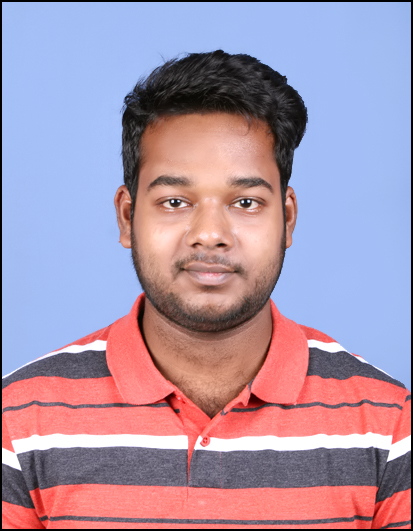
\includegraphics[height=2cm]{Resume_pic}
\end{figure}

%objective
\vspace{3mm}
\textbf{OBJECTIVE : }
To prove my skills and expertise in the area of my interest and adding value to my personal  goals with my zeal and strong determination to learn and perform better every time.

%achivements
\vspace{5mm}
\textbf{ACHIVEMENTS : } 
\vspace{1mm}\\
\begin{enumerate}
\item 1st Position in Embedded Hardware Modeling -Repository Inspection, Sankalp 2018 Techfest, NIST Berhampur, 02/2018.
\item 2nd  Position in the event, Aciequor,National Students Space Challenge, ISRO at IIT-Kharagpur, 10/2018

\item 3rd position in Nutty Squirrel Theme,e-Yantra Robotics Competition 2019,IIT-Bombay
\item Qualifier in DST and Texas Instruments India Innovation Challenge Design Contest 2018, IIM Bangalore
\end{enumerate}

%trainings and internships
\vspace{3mm}
\textbf{TRAINING AND INTERNSHIP : } 
\begin{itemize}
	\item Certification course on Embedded systems(50 hours), at CTTC,Bhubaneswar, 06/2018
	\item Certification course on  Programmable Logic Controller (50 hours), at CTTC,Bhubaneswar, 06/2018
          \item Attended 1 day Workshop on Internet of Things(IOT), at IIT-Kharagpur, by Robonext 07/2017
          \item  Attended 1 day workshop on Manual Robotics organized by NIST ROBOTICS Club, at  NIST,02/ 2017
\end{itemize}

%technical skills
\vspace{3mm}
\textbf{TECHNICAL SKILLS : } 
\begin{itemize}
	\item Simulation Software: PSPICE, TINA, Microsoft Office, Proteus 8.0, Keil microvision, Atmel Studio 6.0, Eagle, Diptrace.
	\item Languages: C, C++
        \item Others: Arduino,8051 board,PCB designing

\end{itemize}

%soft skills
\vspace{3mm}
\textbf{SOFT SKILLS : } 
\begin{itemize}
	\item  Leadership,  Practical  and Logical Approach, Dedication, Team Work, Strong Work Ethic

\end{itemize}


\end{document}



